\section{Zusätzliche Eigenschaften eines Actors}
Die Definition des Actor-Model unter \ref{actor:definition} wird durch gängige implementierungen davon noch durch einige Eigenschaften erweitert \citep{Vernon2015ReactiveAkka}. Diese sind zwar nicht direkt der Definition eines Actors, wie von \cite{Hewitt1973AIntelligence} und \cite{Agha1985ActorsSystems} zuordenbar, sind aber für das Verständnis moderner Anwendungen mit dem Actor-Model von Bedeutung.
\subsection{Hierarchischer Actor Baum}
Actors können ihre Vorteile erst ausspielen wenn sie sich in einem Actor-System (siehe \ref{act:actorSystem}) befinden. Jedoch ist dadurch nicht definiert wie sich das Actor-System organisiert. Im Prinzip ist ein Actor-System eine unbegrenzte Anzahl an unterschiedlichen Actors die untereinander Kommunizieren. Durch die Anwendung einer Hierarchischen Struktur wird in diese Menge eine Struktur gebracht. \\
Erstellt ein Actor, durch die Abarbeitung einer Nachricht, einen neuen Actor, so ist dieser neue Actor ein \textit{Child} des Erstellers. Der Ersteller selber wird dann als \textit{Parent} des neuen Actors (\textit{Child}) betrachtet. Durch dieses Muster kann ein Actor-System als ungerichteter Baum dargestellt werden da jeder Actor maximal einen \textit{Parent} haben kann und eine unbegrenzte Anzahl an \textit{Childs} besitzen kann. \\
In der Abbildung \ref{fig:actor:actorHierarchySample}, ist eine Hierarchie eines kleines Actor-Systems zu sehen. Das Abgebildete System besteht aus 7 Actors wobei drei Actors als \textit{Parent} fungieren und bis zu drei \textit{Childs} besitzen. 
\begin{figure}
    \centering
    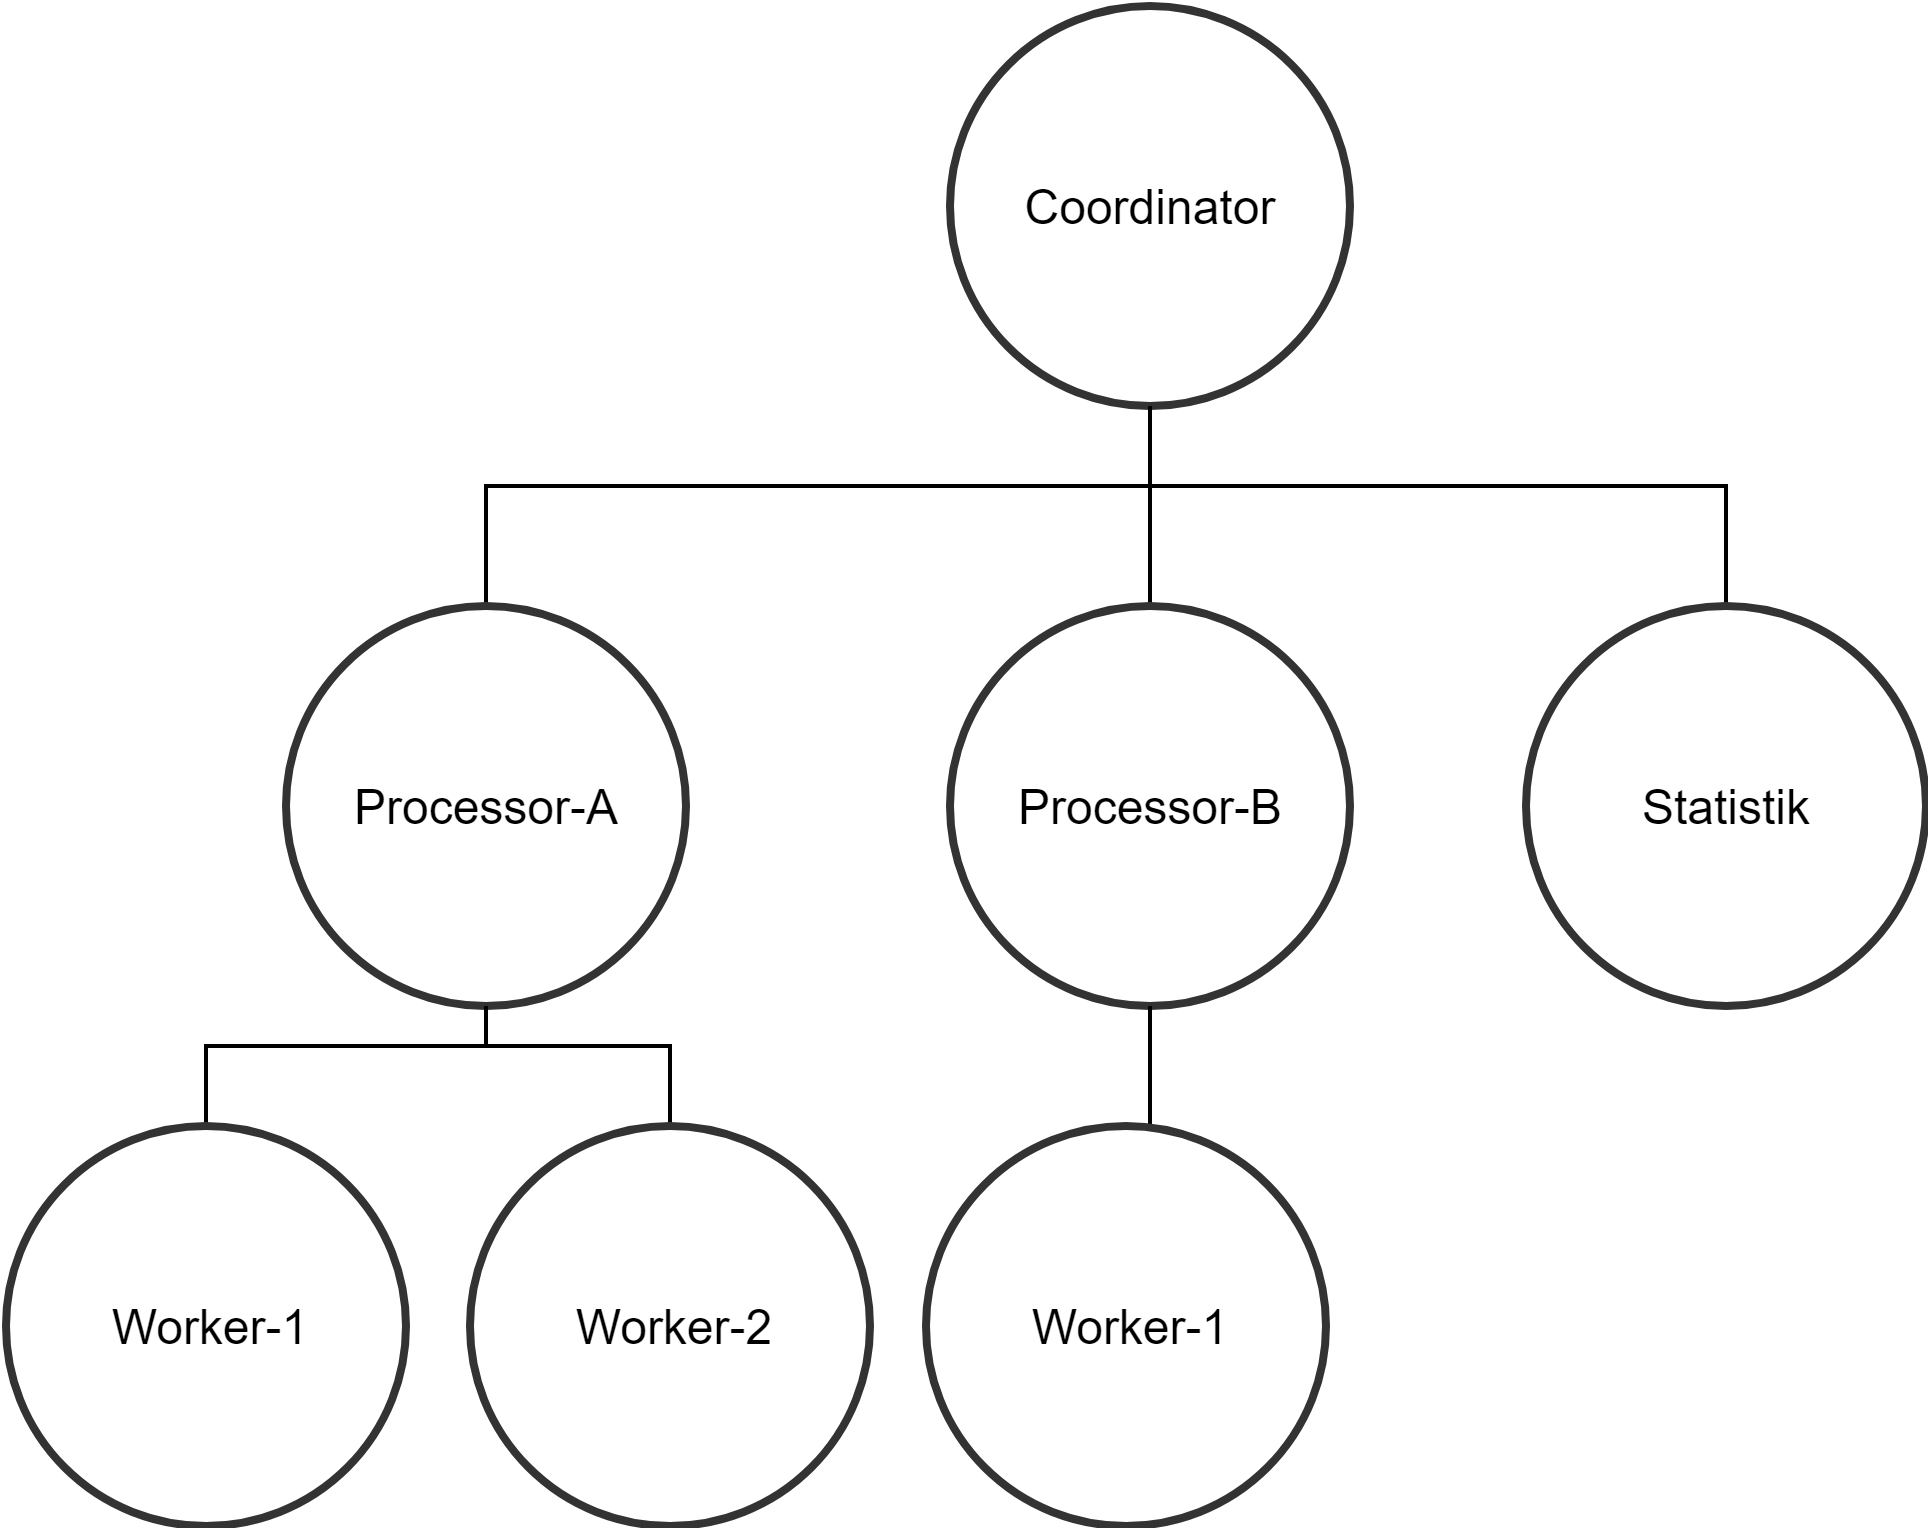
\includegraphics[width=0.6\linewidth]{gfx/actor/actorHierarchy}
    \caption{Ein Beispiel eines Actor-Hierarchie-Baumes}
    \label{fig:actor:actorHierarchySample}
\end{figure}

\subsection{Supervision}\label{actor:supervision}
Damit die im \textit{Reactive Manifest (siehe \ref{reactiveManifesto})} geforderte Bedingung \textit{Wiederstandsfähigkeit} zu erfüllen, bieten Actor Frameworks, wie beispielsweise \textit{Akka} oder \textit{Orleans} (siehe nähere Framework Beschreibung unter \ref{sec:ActorFrameworks}) ein Fehlerhandling welches \textit{Supervision} genannt wird. Das, unter anderem in \cite{sargent2016play} beschriebene, Vorgehen ermöglicht es, mögliche Fehlerquellen zu kapseln und beim Auftretten eines Fehlers während der Laufzeit denn Fehler unabhängig vom Rest des Systemes zu lösen.\\
Das Beispiel in Abbildung \ref{fig:actor:actorHierarchySample}, enthält beispielsweise einen Prozessor Actor \textit{Processor-A}, welcher selber zwei \textit{Childs} hat. Wenn es nun in einem der zwei \textit{Child}-Actors zu einem Fehler kommt, sollte der übergeordnete Actor \textit{Coordinator} im Idealfall nichts davon nichts mitbekommen. Daher kann in diesem Beispiel aus den zwei untersten Actors, wie in Abbildung \ref{fig:actor:actorHierarchySupervison} dargestellt, ein \textit{Error Kernel} gebildet werden. Wenn innerhalb dieses \textit{Kernels} ein Fehler auftritt, wird der \textit{Parent}, was in dem Beispiel der Actor \textit{Processor-A} ist, über den Fehler benachrichtigt, und kann dann darauf entsprechend reagieren. Alle anderen Actors im System bekommen von diesem Vorgehen nichts mit, und Arbeiten ohne Unterbrechung weiter. \\
\begin{figure}
    \centering
    \begin{minipage}{.4\textwidth}
        \centering
        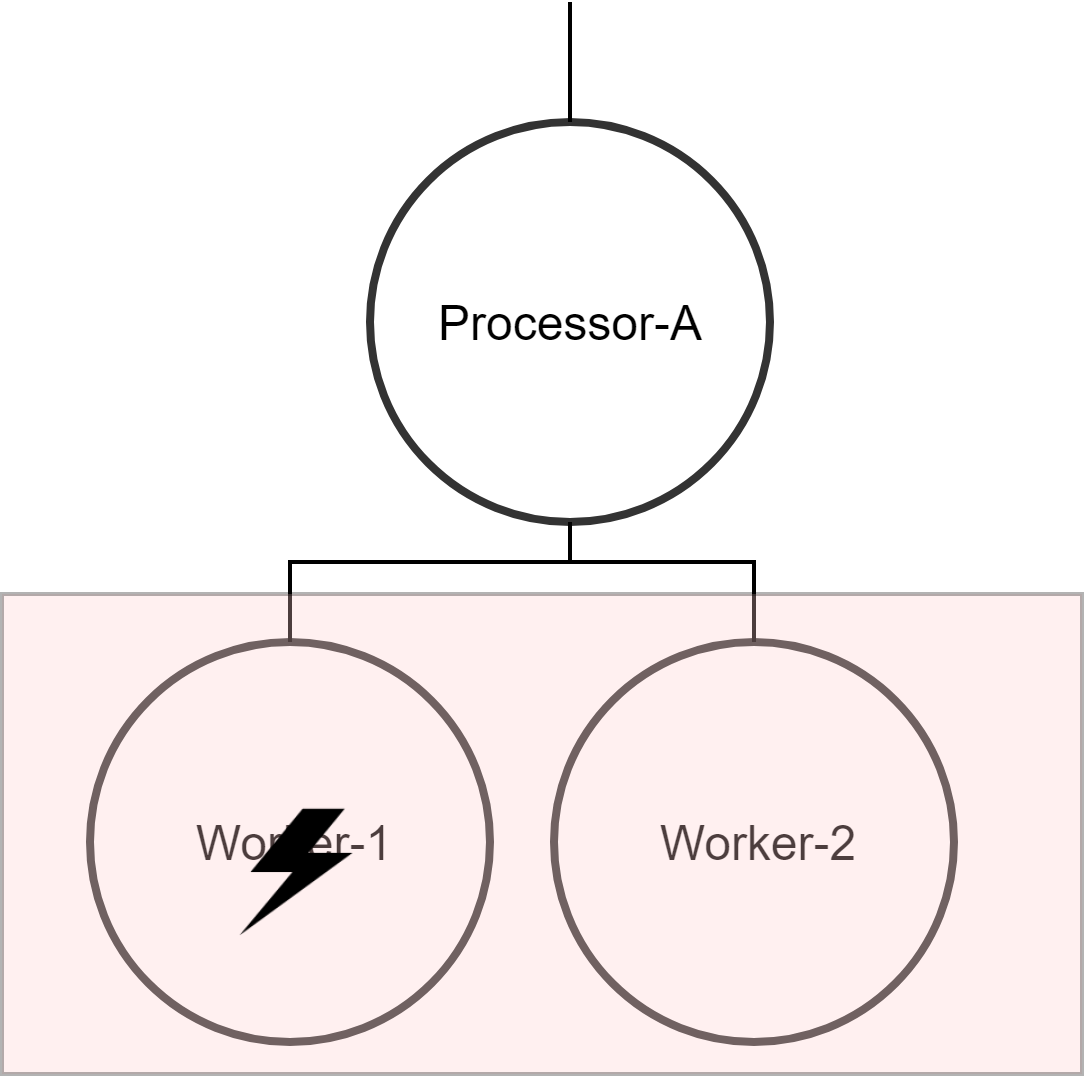
\includegraphics[width=\linewidth]{gfx/actor/actorHierchyErrorKernel}
        \caption{Ein Teil der Hierarchie aus Abbildung \ref{fig:actor:actorHierarchySample} wird ein \textit{Error-Kernel} zugewiesen.}
        \label{fig:actor:actorHierarchySupervison}        
    \end{minipage}%
    \begin{minipage}{.1\textwidth}
    \end{minipage}%
    \begin{minipage}{.5\textwidth}
      \centering
      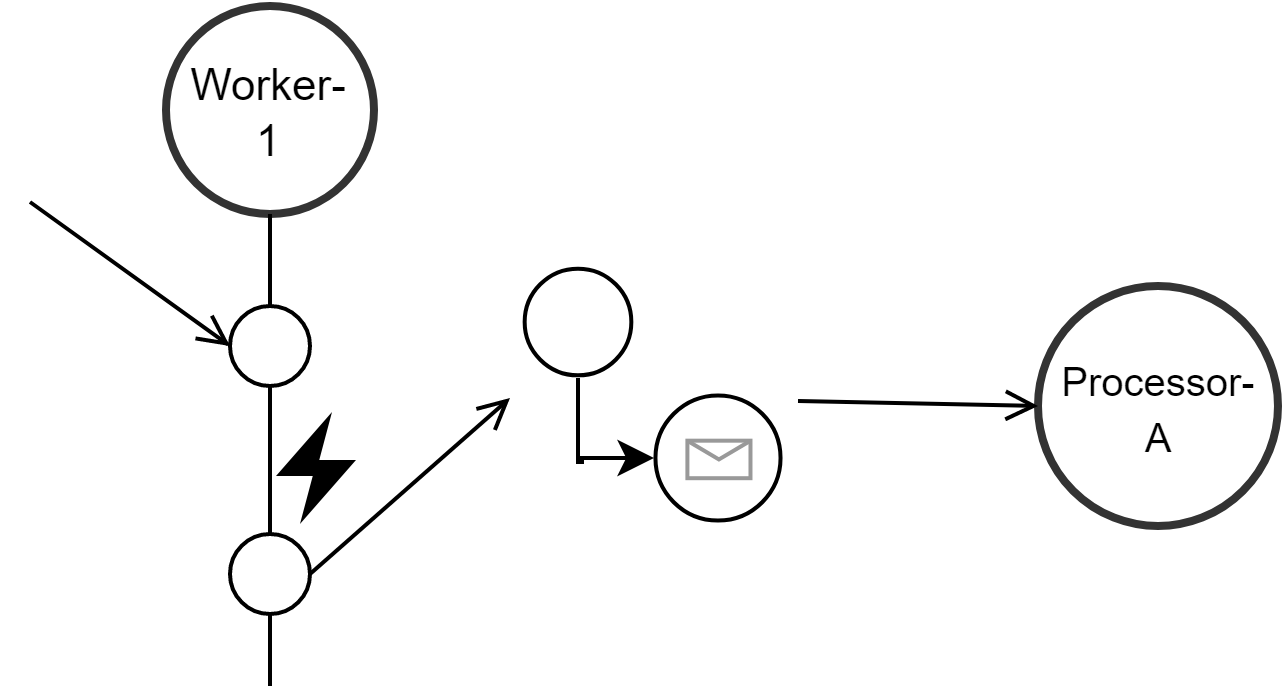
\includegraphics[width=\linewidth]{gfx/actor/actorSupervisionMessageExample}
      \caption{Nachrichten Austausch an den Supervisor des in Abbildung \ref{fig:actor:actorHierarchySupervison} definiterten \textit{Error-Kernel}.}
      \label{fig:actor:actorHierarchySupervisonMessaging}
    \end{minipage}
\end{figure}  

\subsection{Location Transparent}\label{actor:locationTransparency}
Eine weitere Eigenschaft welche etliche Implementierungen dem \textit{Actor-Model} hinzufügen, ist eine nicht gekoppelte Beziehung zwischen den Actoren. Wie in Abschnitt \ref{actor:definition} erklärt, benötigt ein Actor für das Senden einer Nachricht an einen anderen Actor dessen Adresse. Mit dem Prinzip der \textit{location Transparenz}, wird die Adresse eines Actors so gestaltet, das sie nicht an einen Bestimmten Prozess oder Rechner gebunden ist. Durch entkoppelung ist es für den sendenden Actor nicht relevant wo sich der Empfänger befindet. \citep{Vernon2015ReactiveAkka} und \citep{sargent2016play}

